\documentclass[12pt,a4paper]{report}

\usepackage{styles/dolgozat}

\usepackage{listings}
\usepackage{styles/cpp}
\usepackage{styles/python}

\usepackage{hyperref}

\usepackage{caption}
\usepackage{subcaption}

\begin{document}

\pagestyle{empty}

{\small
Miskolci Egyetem \hfill Miskolci Egyetem

Gépészmérnöki és Informatikai Kar \hfill Gépészmérnöki és Informatikai Kar

Általános Informatikai Intézeti Tanszék \hfill \hfill Alkalmazott Matematikai Intézeti Tanszék}

{\large
\begin{center}
\vglue 1.5truecm

\includegraphics[scale=0.15]{images/me_logo.png}\\
\end{center}}

\vglue 1.5truecm

{\huge
\begin{center}
\textbf{A szakdolgozat címe}
\end{center}}

\vspace*{1cm}

\begin{center}
\LARGE \textbf{Szakdolgozat}
\end{center}

\vspace*{2.5truecm}

{\large
\hspace{6.5cm} \textbf{Készítette}:

%\vskip 2mm

\hspace{6.5cm} \textbf{Név}: Szakdolgozó Neve

%\vskip 1mm

\hspace{6.5cm} \textbf{Neptunkód}: \texttt{NPTNCD}

%\vskip 1mm

\hspace{6.5cm} \textbf{Szak}: Mérnökinformatikus BSc

%\vskip 1mm

\hspace{6.5cm} Korszerű web technológiák szakirány
}

\newpage


\newpage

\pagestyle{empty}

\vspace*{1cm}  
\begin{center}
\large\textsc{\bfseries Eredetiségi Nyilatkozat}
\end{center}
\vspace*{2cm}  

Alulírott \textbf{Szakdolgozó Neve}; Neptun-kód: \texttt{N3P7UN} a Miskolci Egyetem Gépészmérnöki és Informatikai Karának végzős Mérnökinformatikus szakos hallgatója ezennel büntetőjogi és fegyelmi felelősségem tudatában nyilatkozom és aláírásommal igazolom, hogy \textit{Szakdolgozat Címe}
című szakdolgozatom saját, önálló munkám; az abban hivatkozott szakirodalom
felhasználása a forráskezelés szabályai szerint történt.\\

Tudomásul veszem, hogy szakdolgozat esetén plágiumnak számít:
\begin{itemize}
\item szószerinti idézet közlése idézőjel és hivatkozás megjelölése nélkül;
\item tartalmi idézet hivatkozás megjelölése nélkül;
\item más publikált gondolatainak saját gondolatként való feltüntetése.
\end{itemize}

Alulírott kijelentem, hogy a plágium fogalmát megismertem, és tudomásul veszem, hogy
plágium esetén szakdolgozatom visszautasításra kerül.

\vspace*{3cm}

\noindent Miskolc, \hbox to 2cm{\dotfill} .év \hbox to 2cm{\dotfill} .hó \hbox to 2cm{\dotfill} .nap

\vspace*{3cm}

\hspace*{8cm}\begin{tabular}{c}
\hbox to 6cm{\dotfill}\\
Hallgató
\end{tabular}

\newpage


\cleardoublepage
\pagenumbering{gobble}
\tableofcontents
\cleardoublepage
\pagenumbering{arabic}

\newpage

\pagestyle{fancy}

\Chapter{Bevezetés}

Ha nekünk nem is, de nagyszüleinknek bizonyára megtalálhatók még régi, szürkeárnyalatos fényképek a fiók mélyén. Az ilyen régi, családi képeket nézegetve keltette fel az érdeklődésemet a dolgozat témaköre. Érdekelt, hogy vajon hogyan tudnánk az ilyen fotókat életre kelteni színek segítségével.

A képek kiszínezése két problémakörre osztható. 
Az első problémakör azon részek meghatározása a képen, amelyek eredetileg azonos színűek lehettek. Ha mi, emberek ránézünk egy képre, ezt könnyen meg tudjuk határozni, viszont a számítógép számára ez már nem ilyen egyszerű. A dolgozatban több módszert is megvizsgálok annak érdekében, hogy minél pontosabban tudjam meghatározni az azonos színű területeket.

A második problémakör az nem más, mint hogy hogyan tudjuk kiszínezni ezeket az összefüggő részeket, és meghatározni azt a színt, amely a legközelebb állhat az objektum eredeti színéhez. Mint az első problémakörnél, nekünk, embereknek ez szintén nem jelent kihívást, hiszen ha látunk például egy banánt egy szürkeárnyalatos képen, tudjuk, hogy valószínűleg sárga színű lehetett. A számítógépnek viszont meg kell tanítanunk, hogy adott tárgyak, adott textúrák milyen színűek, és ebből megpróbálja kitalálni hogy a szürkeárnyalatos képen szereplő tárgy, textúra milyen színű lehet.

A dolgozat elején bemutatásra kerülnek a probléma megoldásához használt általános eszközök. Azt követően a K-means klaszterező eljárás segítségével láthatjuk, hogy hogyan lehet a képet szegmensekre, régiókra bontani. Ezt a szegmentálás egy érdekes megközelítéseként a szuper pixeles vizsgálatok követik. Végül a képek egyes részeinek színére vonatkozó becslési eljárások következnek.

\Chapter{Koncepció}

\Section{A fejezet célja}

Ez a fejezet még nem a saját eredményekkel foglalkozik, hanem bemutatja, mi a problémakör, milyen módszerekkel, milyen eredményeket sikerült elérni eddig másoknak.

A hivatkozások jelentős része ehhez a fejezethez szokott kötődni.
(Egy hivatkozás például így néz ki \cite{coombs1987markup}.)
Ez szintén egy példa internetes hivatkozásra, a CSS szabvány kapcsán \cite{css}.
Itt lehet bemutatni a hasonló alkalmazásokat.

\Section{Tartalom és felépítés}

A fejezet tartalma témától függően változhat. Az alábbiakat attól függően különböző arányban tartalmazhatják.
\begin{itemize}
\item Irodalomkutatás. Amennyiben a dolgozat egy módszer kidolgozására, kifejlesztésére irányul, akkor itt lehet részletesen végignézni (módszertani vagy időrendi bontásban), hogy az eddigiekben milyen eredmények születtek a témakörben.
\item Technológia. Mivel jellemzően kutatásról vagy szoftverfejlesztésről van szó, ezért annak a jellemző elemeit, technikai részleteit itt kell bemutatni.
Ez tehát egy módszeres bevezetés ahhoz, hogy ha valaki nem jártas a témakörben, akkor tudja, hogy a dolgozat milyen aktuálisan elérhető eredményeket, eszközöket használt fel.
\item Piackutatás. Bizonyos témáknál új termék vagy szolgáltatás kifejlesztése a cél.
Ekkor érdemes annak alaposan utánanézni, hogy aktuálisan milyen eszközök érhetők el a piacon.
Ez szoftverek esetében a hasonló alkalmazások bemutatását, táblázatos formában történő összehasonlítását jelentheti.
Szerepelhetnek képek és észrevételek a viszonyításként bemutatott alkalmazásokhoz.
\item Követelmény specifikáció. Külön szakaszban érdemes részletesen kitérni az elkészítendő alkalmazással kapcsolatos követelményekre.
Ehhez tartozhatnak forgatókönyvek (\textit{scenario}-k).
A szemléletesség kedvéért lehet hozzájuk képernyőkép vázlatokat is készíteni, vagy a használati eseteket más módon szemléltetni.
\end{itemize}

\Section{Amit csak említés szintjén érdemes szerepeltetni}

Az olvasóról annyit feltételezhetünk, hogy programozásban valamilyen szinten járatos, és a matematikai alapfogalmakkal sem ebben a dolgozatban kell megismertetni.
A speciális eszközök, programozási nyelvek, matematikai módszerekk és jelölések persze jó, hogy ha említésre kerülnek, de nem kell nagyon belemenni a közismertnek tekinthető dolgokba.

\Chapter{Általános információk (?)}

Ebben a fejezetben néhány általános információ található, amik a dolgozat teljes egészére érvényesek.

\Section{Felhasznált képek}

A teszteléshez csendéletekről készült képeket gyűjtöttem az unsplash nevezetű weboldalról. \cite{unsplash}
A csendéleteken a tárgyak intenzitása jól elkülönül a háttér intenzitásától így egyszerűbben lehet rajta szegmentálást végrehajtani.
A képek nevei a 0 és 5 közötti számok, pl. 0.jpg.

\Section{Képek feldolgozása}

A képek feldolgozása során előfordulnak olyan lépések, műveletek amelyeket több ponton is megismételtem. Ezeket ebben a bekezdésben szeretném bemutatni, a későbbiekben nem térek ki rájuk részletesen. 
A képfeldolgozáshoz az opencv-python könyvtárat használtam.

\SubSection{Betöltés}

A képeket két módon töltöm be a további feldolgozásra:
\begin{itemize}
\item színesen
\item szürkeárnyalatosan
\end{itemize}
Ehhez két külön metódust készítettem:
\begin{itemize}
\item \texttt{load\_image\_rgb}
\item \texttt{load\_image\_grayscale}
\end{itemize}
Ezek eleinte minden notebookban ismétlődtek, majd a kutatás későbbi szakaszában kiszerveztem őket a \texttt{commonmethods} nevű saját készítésű python librarybe amiről részletesebben a következő alfejezetben írok.

A szürkeárnyalatos kép betöltését a következő kódrészlet tartalmazza.
\begin{python}
import cv2

def load_image_grayscale(name):
    """
    Loading the image from the images folder using opencv-python
    :param name: the name of the image I want to load,
        the method doesn't need the path or the extension
    :return: the loaded image in grayscale color
    """
    image = cv2.imread('../images/' + format(name) + '.jpg')
    image = cv2.cvtColor(image, cv2.COLOR_BGR2GRAY)

    return image
\end{python}
A színes kép betöltése annyiban különbözik, hogy a cv2.COLOR\_BGR2GRAY helyett cv2.COLOR\_BGR2RGB szerepel.

Mind a két metódus a kép nevét várja bemenetként. Mivel a tesztelés során használt képek mindegyike JPG típusú így a kiterjesztést a metódus automatikusan hozzákapcsolja.

\SubSection{Átméretezés}

Átméretezésre a \texttt{resize\_image} metódust készítettem, amelynek a forráskódja a következő:
\begin{python}
import cv2

def resize_image(image, wanted_height) :
    """
    Resizing the image for the given height,
    without disortion, using opencv-python
    :param image: the image that I want to resize
    :param wanted_height: the height in pixel that
        I want to have in the resized image
    :return: the resized image
    """
    height = image.shape[0]
    # calculating the amount with I need to change the width
    scale_percent = height / wanted_height
    width = int(image.shape[0] / scale_percent)
    dim = (width, wanted_height)

    resized_image = \
        cv2.resize(image, dim, interpolation = cv2.INTER_AREA)

    return resized_image
\end{python}
Bemenetként magát a képet várja és azt a méretet px-ben, amire a magasságot szeretnénk változtatni. Hogy ne torzuljon a kép, kiszámítok egy arányt a paraméterként kapott méretből és a kép magasságából, majd ezzel az aránnyal csökkentem a kép szélességét.

\Section{Közös metódusok kiszervezése}

Írni a saját Python libraryről, hogyan kell használni stb. \cite{pythonlibrary}

\Section{Tesztelési környezet}

A programkódok tesztelését minden esetben az otthoni számítógépemen végeztem aminek a paraméterei a következők:
\begin{itemize}
\item Processzor: Intel(R) Core(TM) i5-9400F CPU 2.90GHz
\item Memória mérete: 16 GB
\item (?) Videókártya: NVIDIA GeForce GTX 1660
\item Operációs rendszer: Windows 10 Enterprise
\end{itemize} 
\Chapter{K-means klaszterezés}

\Section{Klaszterezés}

Ahhoz, hogy szürkeárnyalatos képeket megfelelően tudjunk kiszínezni, első lépésként meg kell határoznunk a kiszínezendő területeket. El kell döntenünk, hogy a kép mely részei tartoznak ugyan ahhoz a színárnyalathoz és melyek nem. Ezek alapján a dolgozat 2 fő részre bontható:
\begin{itemize}
\item képszegmentálás
\item szegmensek kiszínezése
\end{itemize}

A képszegmentálás célja az, hogy a képen lévő különböző célterületeket elkülönítse, a klaszterezés célja pedig az azonos tulajdonságokkal rendelkező objektumok közös kategóriába sorolása ahol az egy kategóriába tartozó objektumok egymáshoz hasonlóak, viszont különböznek a többi kategóriában lévő objektumoktól.

A két módszer célja lényegében megegyezik egymással. Ahhoz hogy a képből ki tudjuk nyerni a megfelelő szegmenseket, valamilyen klaszterezési eljárást kell alkalmaznunk.

A klaszterezési algoritmusokat a következő módon tudjuk csoportosítani \cite{clustering}:
\begin{itemize}
\item hierarchikus: a korábban létrehozott klaszterek felhasználásával találja meg az egymást követő klasztereket
    \begin{itemize}
    \item agglomeratív (bottom-up): minden egyes elemet különálló klaszterként kezel és azokat nagyobb klaszterekbe egyesíti
    \item osztó (top-down): a teljes halmazból indul ki és azt kisebb klaszterekre osztja
    \end{itemize}
\item particionáló: egyszerre határozza meg az összes klasztert
\item rács alapú: a teret véges számú cellára kvantálja amelyek egy rácsszerkezetet alkotnak, és ezeken hajtja végre a klaszterezést
\item modell alapú: megpróbálja az adatokat optimálisan ráilleszteni valamilyen matematikai modellre
\end{itemize}

A kutatások során az egyik legnépszerűbb particionáló klaszterezést használtam, a k-means klaszterezést.

\Section{K-means módszer}
A klaszterezés célja, hogy egy adathalmazt diszjunkt részhalmazokra (klaszterekre) ossza fel méghozzá úgy, hogy a klaszterezési kritérium optimális legyen. A legelterjedtebb klaszterezési kritérium az egyes adatpontok, és az azokat tartalmazó részhalmaz súlypontja (klaszterközéppont) közötti négyzetes Euklidészi távolságok összege. Ezt hívják klaszterezési hibának és ennek az optimalizálása a cél. \cite{kmeans}

A K-means algoritmus lokálisan optimális megoldásokat talál, figyelembe véve a klaszterezési hibát. Ez egy gyors, iteratív módszer aminek az algoritmusa a következő \cite{tomatoleaf}:
\begin{enumerate}
\item lépés: véletlenszerűen kiválaszt $K$ darab klaszterközéppontot
\item lépés: meghatározza az egyes pontok távolságát a középpontoktól valamilyen távolságfüggvény szerint, majd besorolja az egyes pontokat a hozzájuk legközelebbi klaszterközéppont kategóriájába
\item lépés: kiszámítja az egyes klaszterek számtani átlagát és az lesz az új klaszterközéppont
\item lépés: megnézi, hogy a klaszterközéppontok helyzetében történt-e változás:
    \begin{enumerate}
    \item ha igen, akkor megismétli az algoritmust a 2. lépéstől
    \item ha nem, akkor megáll az algoritmus, mivel megtalálta az optimális klasztereket
    \end{enumerate}
\end{enumerate}

A módszer nagy előnye hogy könnyen megvalósítható, viszont az algoritmusból láthatóak a módszer hátrányai is.

A végső klaszterezés a kezdeti klaszterközéppontok helyzetétől és a $K$ értékétől függ. A $K$ a klaszterek számát jelöli, és ezt az értéket nekünk kell meghatároznunk még a klaszterezési algoritmus futása előtt. Két K-means futási eredmény nagyban különbözhet, hiszen a középpontok kezdeti értéke véletlenszerű. Ahhoz, hogy ténylegesen az optimális eredményt kapjuk, érdemes az algoritmust többször futtatni.

Az optimális klaszterszám meghatározására több módszert is kipróbáltam, ezeket a \ref{optimal_cluster_number}. alfejezetben ismertetem.

A kutatásom során a \texttt{opencv-python} könyvtárban található K-means metódust használtam. Mivel a szegmentálás ez egyik fő eleme a kutatásomnak, így ezt is kiszerveztem az általam készített \texttt{commonmethods} könyvtárba \texttt{kmeans\_segmentation} néven. A következő kódrészletben látható az általam megírt algoritmus.
\begin{python}
def kmeans_segmentation(values, k):
    """
    Segmenting the given values using opencv-python's k-means method
    :param values: the values at which I want to perform segmentation
    :param k: the number of the clusters
    :return: the compactness, the labels and
        the centers from the k-means method
    """
    values = np.float32(values)

    criteria = \
        (cv2.TERM_CRITERIA_EPS + cv2.TERM_CRITERIA_MAX_ITER, 100, 0.2)

    compactness, labels, (centers) = cv2.kmeans(
        values,
        k,
        None,
        criteria,
        10,
        cv2.KMEANS_RANDOM_CENTERS)

    labels = labels.flatten()

    return compactness, labels, (centers)
\end{python}

Bemeneti paraméterként a szegmentálni kívánt értékeket és a klaszterek számát várja a metódus. Első lépésként átalakítom a kapott értékeket a \texttt{cv2.kemans} metódusnak megfelelő formátumra.

Maga a \texttt{cv2.kmeans} a következő paramétereket várja \cite{kmeans_opencv}:
\begin{itemize}
\item \texttt{samples}: Egy tömb amely \texttt{np.float32} típusú és a jellemzők külön oszlopokban helyezkednek el.
\item \texttt{nclusters(K)}: A klaszterek száma.
\item \texttt{bestLabels}: Bemeneti/kimeneti tömb amely minden mintához eltárolja a klaszterindexet.
\item \texttt{criteria}: Ez az iterációs kritérium. Ha ez teljesül, akkor az algoritmus megáll. A típusa tuple ami 3 paramétert tartalmaz:
    \begin{itemize}
    \item \texttt{type}: A leállási kritériumnak a típusa, 3 flagje (?) létezik:
        \begin{itemize}
        \item \texttt{cv.TERM\_CRITERIA\_EPS}: Akkor áll meg az algoritmus, ha elértük a kívánt pontosságot.
        \item \texttt{cv.TERM\_CRITERIA\_MAX\_ITER}: Akkor áll meg az algoritmus, ha elértük a maximális iterációk számát.
        \item \texttt{cv.TERM\_CRITERIA\_EPS} + \texttt{cv.TERM\_CRITERIA\_MAX\_ITER}: Akkor áll le az algoritmus, ha az előző két flag közül bármelyik bekövetkezik.
        \end{itemize}
    \item \texttt{max\_iter}: Az iterációk maximális száma.
    \item \texttt{epsilon}: Az elvárt pontosság.
    \end{itemize}
\item \texttt{attempts}: Azt adjuk meg, hogy hányszor fusson le az algoritmus különböző klasztereket eredményezve. A visszatérési érték a legoptimálisabb klaszter lesz.
\item \texttt{flags}: A kezdeti középpontok felvételének a módját tudjuk megadni. Általában 2 típusa van:
    \begin{itemize}
    \item \texttt{cv.KMEANS\_PP\_CENTERS}: Arthur és Vassilvitskii kmeans++ középpont inicializálási metódusát használva határozza meg a középpontokat.
    \item \texttt{cv.KMEANS\_RANDOM\_CENTERS}: Random határozza meg a középpontokat.
    \end{itemize}
\end{itemize}

A paramétereket úgy állítottam be hogy 10 alkalommal fusson le az algoritmus, és a klaszterek kezdő középpontját random határozza meg. Ezen kívül az algoritmus megáll ha eléri vagy a maximális iterációk számát ami 100, vagy a megfelelő pontosságot ami 0.2.

Ezeket a paramétereket a \cite{kmeans_opencv} dokumentáció alapján határoztam meg, egyedül a pontosságot, az \texttt{epsilon} értékét állítottam kisebbre mint a dokumentációban szereplő érték.

A k-means módszert kétféleképpen teszteltem le. Először csak a kép intenzitását vettem figyelembe, és az összes képpontot átadtam az algoritmusnak szegmentálásra. Ezek után feature vektorokat hoztam létre azzal a szándékkal, hogy textúra alapján végezzem a szegmentálást. A vizsgálatok eredménye a következő fejezetekben található.

\Section{Klaszterezés intenzitás alapján}

Az intenzitás alapú szegmentálás során nem volt másra szükségem, csak a kép pixeleinek az értékére. A szürkeárnyalatos kép pixeleit egy $n\times1$ méretű, a színes képek pixeleit pedig egy $n\times3$ méretű tömbbé alakítottam át. Erre a \texttt{numpy} csomagban található \texttt{reshape} metódust használtam a következő kódrészletben látható módon.
\begin{python}
#grayscale image
grayscale_pixel_values = grayscale_image.reshape((-1, 1))

#rgb image
rgb_pixel_values = rgb_image.reshape((-1, 3))
\end{python}

A megkapott értékeket adtam át a \texttt{kmeans\_segmentation} metódusnak.

A szegmentálás eredményei különböző számú klaszterekre a \ref{fig:kmenas_grayscale}. ábrán látható szürkeárnyalatos képek esetén, és a \ref{fig:kmenas_rgb}. ábrán látható színes képek esetén. Mind a két esetben 2, 4, és 8 értékeket állítottam be a klaszterek számának.

A szegementált képeket a \texttt{kmeans\_segmentation} által előállított \texttt{labels} és \texttt{centers} értékek segítségével rajzolom ki. Az egy kategóriába tartozó pixeleket kiszínezem a kategóriájuk középpontjával megegyező színnel a következő kódrészletben látható módon.

\begin{python}
centers = np.uint8(centers)
segmented_image = centers[labels.flatten()]
segmented_image = segmented_image.reshape(image.shape)
\end{python}

Először a középpontok értékét \texttt{np.float32} típusról átalakítom integer típusra, majd a \texttt{labels} értékek alapján létrehozom a szegmentált kép pixeleit tartalmazó tömböt. Ez a tömb egy dimenziós lesz, így kirajzolás előtt átalakítom az eredeti képpel megegyező formátumra.

\begin{figure}[h]
\centering
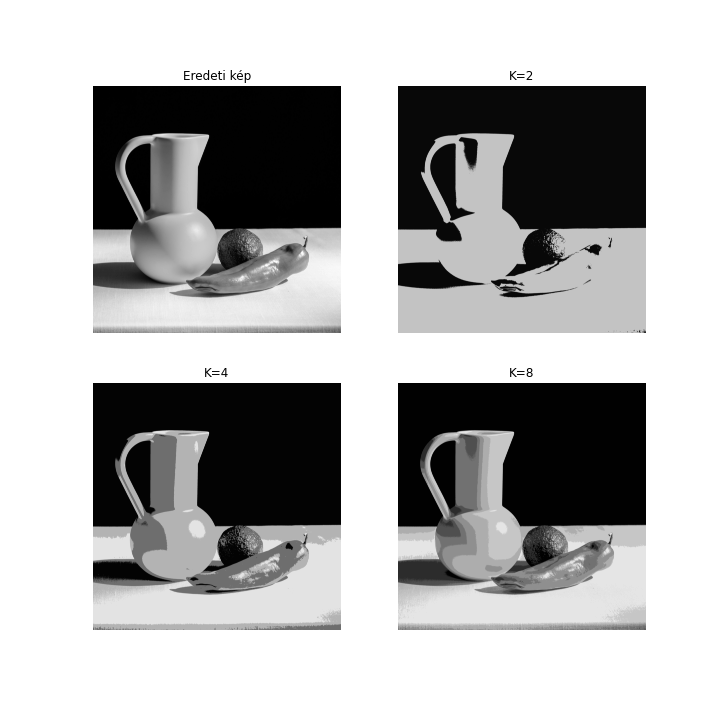
\includegraphics[scale=0.6]{images/kmeans_grayscale.png}
\caption{K-means módszer futási eredménye szürkeárnyalatos kép esetén, különböző klaszterszámokra}
\label{fig:kmenas_grayscale}
\end{figure}

\begin{figure}[h]
\centering
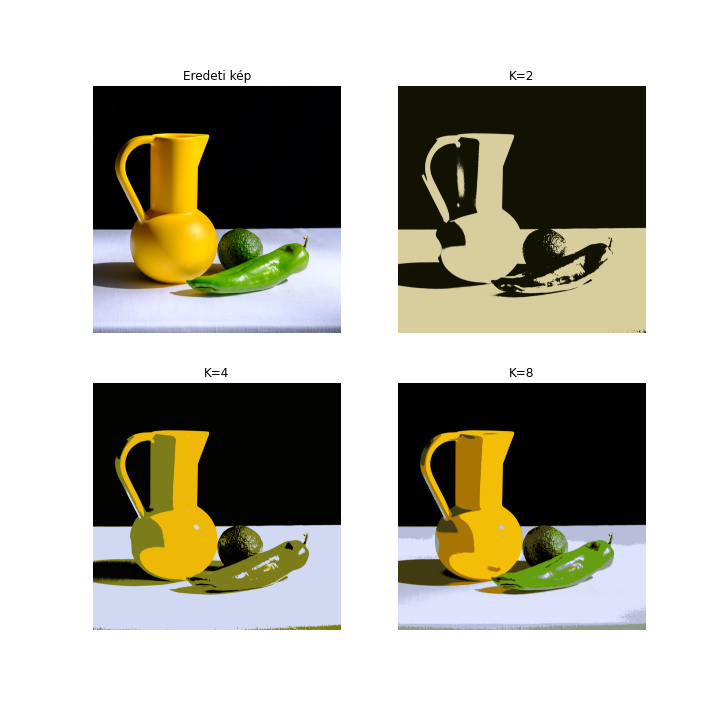
\includegraphics[scale=0.6]{images/kmeans_rgb.png}
\caption{K-means módszer futási eredménye színes kép esetén, különböző klaszterszámokra}
\label{fig:kmenas_rgb}
\end{figure}

A módszer vizsgálata során kitértem a futási időre is. Logikusan következik, hogy a képek méretének növelésével, vagy a klaszterek számának növelésével a módszer futási ideje is növekszik. A \ref{fig:kmenas_runtime_cluster}. és a \ref{fig:kmenas_runtime_size}. ábrákon található ezeknek a vizsgálatoknak az eredménye.

Jól látható, hogy a klaszterek számának növelésével a futási idő nem minden alkalommal növekszik, viszont a képek méretének növelésével a futási idő növekedése folyamatos. Emellett az is megfigyelhető, hogy sem a legnagyobb vizsgált klaszterszám (10), sem a legnagyobb vizsgált képméret (768px) esetén nem éri el a futási idő a 0.5 másodpercet, tehát az algoritmus futási ideje még ezekben az esetekben is gyors.

\begin{figure}[h]
\centering
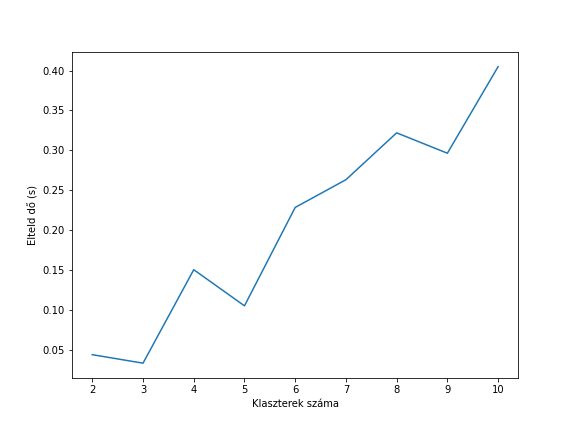
\includegraphics[scale=0.7]{images/kmeans_runtime_cluster.png}
\caption{K-means módszer futási ideje különböző klaszterszámokra}
\label{fig:kmenas_runtime_cluster}
\end{figure}

\begin{figure}[h]
\centering
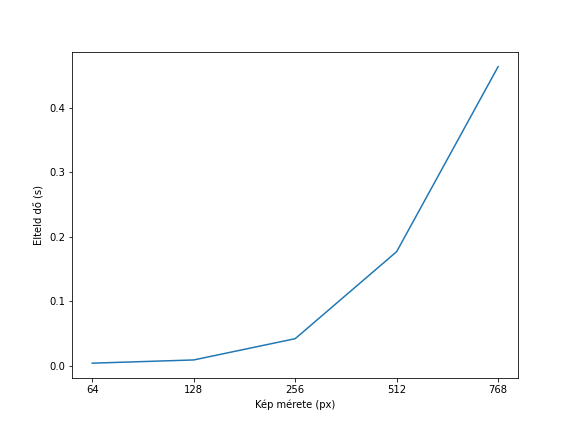
\includegraphics[scale=0.7]{images/kmeans_runtime_size.png}
\caption{K-means módszer futási ideje különböző méretű képekre}
\label{fig:kmenas_runtime_size}
\end{figure}

A futási idők után megvizsgáltam, hogy vajon különböző méretű képekre mennyire pontos a klaszterezés. A klaszterek számának 4-et adtam meg, a klaszterezést pedig elvégeztem 64px, 128px, 256px és 512px méretű képekre. A futási eredményeket a \ref{fig:kmenas_picture_sizes}. ábra tartalmazza.

Egyértelműen látszik, hogy már a legkisebb, 64px méretű képen is ugyanazokat a klasztereket találja meg mint a legnagyobb, 512px méretű képen.

\begin{figure}[h]
\centering
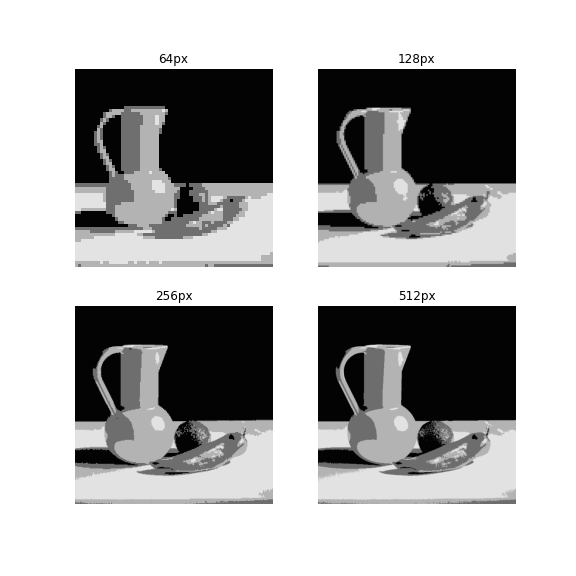
\includegraphics[scale=0.7]{images/kmeans_picture_sizes.png}
\caption{K-means módszer futási eredménye különböző méretű képekre}
\label{fig:kmenas_picture_sizes}
\end{figure}

\Section{Klaszterezés textúra alapján}

Az intenzitás alapú klaszterezés során az objektumokat egymástól nem igazán lehetett megkülönböztetni, így másik módszert próbáltam alkalmazni. 

A textúra alapú klaszterezés során úgynevezett feature vektorokat készítettem és ezeket adtam át a \texttt{kmeans\_segmentation} metódusomnak. A feature vektor egy $n\times px^2$ méretű tömb, ami $n$ darab az eredeti képből kivágott $px \times px$ méretű ablakot tartalmaz. Ezek az ablakok tartalmazzák a különböző textúrákat. A szegmentálás során a \texttt{k-means} módszer megpróbálja megtalálni az egymáshoz legjobban hasonlító ablakokat, vagyis textúrákat.

Egy ablak kinyerését a következő kódrészletben látható \texttt{get\_window} metódus végzi el.
\begin{python}
import numpy as np

def get_window(image, row_number, column_number, px):
    """
    Method for getting the px x px sized window from the image.
    :param image: the image that I want to get the window from
    :param row_number: the row where the window left corner pixel 
        should start
    :param column_number: the column where the window left corner pixel 
        should start
    :param px: the width and height of the window
    :return: the px x px sized window from the image
    """
    window = np.zeros((px, px))

    for i in range(0, px):
        column = np.zeros((px))
        for j in range(0, px):
            column[j] = image[row_number+i][column_number+j]
        window[i] = column

    return window
\end{python} 

A függvény bemenetként a képet, az ablak méretét, és az ablak bal felső pixelének az $x, y$ koordinátáit várja \texttt{column\_number} és \texttt{row\_number} néven. 

Első lépésként létrehozok egy $px \times px$ méretű tömböt amit feltöltök nullákkal, majd indítok két egymásba ágyazott for ciklust nullától $px$ méretéig. A külső ciklusban az oszlopokat hozom létre, majd a belső ciklussal végig haladok az oszlopban található pixelek értékein, és lementem őket. Az így kapott oszlopokat összefűzve megkapom a képemből kinyert ablakot.

A függvény által meghatározott ablakokra példa a \ref{fig:window_example}. ábrán található. A \texttt{px} értékének 15-öt állítottam be, az ablakok kezdőértékei pedig a képek tetején szerepelnek. Az eredeti kép, az 5.jpg látható a bal felső ábrán. Az ablakok a képnek a különböző textúráit mutatják be, mindegyik textúra felett megtalálható annak az objektumnak a neve amiről származik. Megfigyelhető hogy amíg a háttér, az avokádó, és a terítő textúrája elég egyedi, addig a kancsó és a paprika textúrája nagyon hasonló egymáshoz. Az ő esetükben szükség lehet az ablakokon kívül más értékekre is (például az intenzitásukra), ami alapján a szegmentálás során meg lehet őket különböztetni.

\begin{figure}[h]
\centering
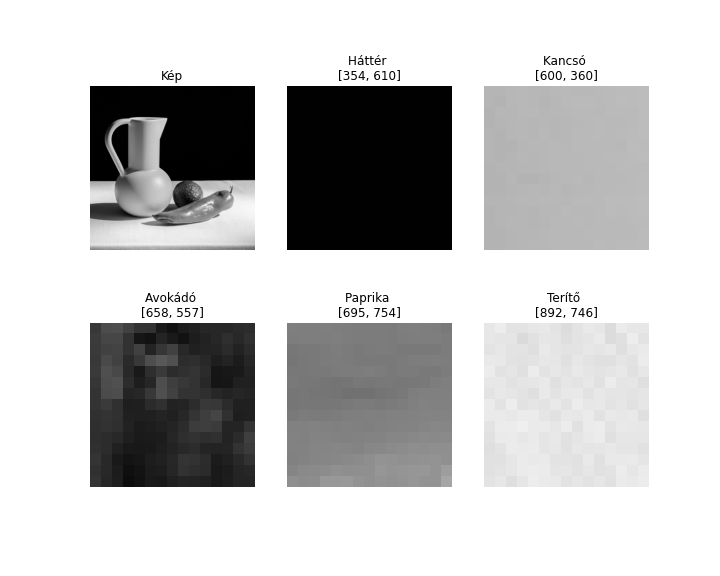
\includegraphics[scale=0.6]{images/window_example.png}
\caption{$15px\times 15px$ méretű minta ablakok a vizsgált képen található különböző textúrákról.}
\label{fig:window_example}
\end{figure}

Ahhoz, hogy a teljes képet szegmentálni tudjam, szükségem van több ilyen $px \times px$ méretű ablakra. Hogy minél nagyobb valószínűséggel lefedjem a képen található összes textúrát, az ablakok helyzetét random határozom meg. Készítettem egy metódust \texttt{get\_window\_values} néven, ami a következő kódrészletben található.
\begin{python}
import numpy as np

def get_window_values(image, window_quantity, px):
    """
    Method for getting random windows from the image, 
    stacked in one vector.
    The resulted vector size will be window_quantity x px*px.
    :param image: the image that i want to get the random windows from
    :param window_quantity: the amount of windows that i want to get
    :param px: the width and height of the windows
    :return: the result, which is the vector created from the windows, 
        and the pixels, an array that contains the start pixels 
        of the windows
    """
    height = image.shape[0]
    width = image.shape[1]

    pixels = np.zeros((window_quantity, 2))

    #get random window start pixels
    x = np.random.randint(0, height-px, window_quantity)
    y = np.random.randint(0, width-px, window_quantity)

    for i in range(window_quantity):
        window = get_window(image, x[i], y[i], px)
        window = window.reshape((1, -1))
        pixels[i] = [x[i], y[i]] #saving the start pixels of the windows

        if i == 0:
            result = np.array(window)
        else:
            result = np.vstack([result, window])

    return result, pixels
\end{python}

A függvény bemeneti paraméterként az ablakok számát és a méretét, ezen kívül azt a képet várja, amin az ablakokat szeretném meghatározni.

Első lépésként létrehozok egy tömböt \texttt{pixels} néven, amiben az ablakok kezdeti pixeleit fogom eltárolni. Ezután a \texttt{numpy} csomag \texttt{random.randint} metódusa segítségével létrehozok \texttt{window\_quantity} mennyiségű, 0 és a kép mérete-px közötti integer számokat. 2 listát kapok, az egyikből kapom meg az $x$, a másikból az $y$ koordinátáit az ablakok kezdő pixeleinek. Egy for ciklus segítségével létrehozok \texttt{window\_quantity} darabszámú ablakot a fentebb említett \texttt{get\_window} függvény segítségével. A megkapott ablakokat átalakítom 1 dimenziós tömbbé, majd hozzáadom a result listához.

Eredményül egy $\texttt{window\_quantity} \times px^2$ méretű tömböt kapok. Ez lesz az a feature vektor, amit átadok a \texttt{kmeans\_segmentation} metódusomnak szegmentálásra. 

A szegmentálás eredményeként minden ablakra kapok egy label értéket. Annak érdekében hogy a pixeleket a megfelelő label szerint tudjam egyszerűen kiszínezni, készítettem egy \texttt{get\_label\_map} nevű metódust amit a következő kódrészlet tartalmaz.

\begin{python}
def get_label_map(height, width, pixels, labels, px):
    """
    Method for getting the label to each pixel of the windows.
    :param height: the height of the image that contains the windows
    :param width: the width of the image that contains the windows
    :param pixels: the starting pixels of the previously 
        calculated windows
    :param px: the width and height of the windows
    :return: an array in the shape of the image, 
        the values are -1 where the pixel is not segmented,
        the labels elswhere
    """
    label_map = np.full((height, width), -1)

    for i in range(len(pixels)):
        for j in range(0, px):
            for k in range(0, px):
                label_map[int(pixels[i][0]+j)][int(pixels[i][1]+k)] =\
                    labels[i]

    return label_map
\end{python} 

A függvény bemeneti paraméterként az eredeti kép méreteit, az ablakok méretét és kezdő pixeleit, ezen kívül a labeleket várja. Első lépésként létrehozok egy tömböt, ami ugyanolyan formájú mint maga a kép, és feltöltöm minden értékét -1-gyel. Ehhez a \texttt{numpy} csomag \texttt{full} függvényét használom. A -1 fogja jelezni, hogy egy pixel még nem kapott labelt. Ezután indítok egy for ciklust ami végig halad az ablakok kezdő pixelein. A kezdő értékektől indulva bejárom a $px \times px$ méretű ablakot, így megkapva az ablak összes pixelét, és minden pixelhez az ablakhoz kapott labelt rendelem hozzá. Eredményként kapok egy olyan térképet, ami a szegmentált pixelnél a labelt, a még nem szegmentált pixelnél pedig -1-et tartalmaz. 

A megkapott szegmensek kirajzolása érdekében készítettem egy \texttt{color\_image} metódust ami a következő kódrészletben látható.

\begin{python}
import cv2
import numpy as np

def color_image(image, label_map):
    """
    Method for colorizing the image based on the label_map.
    :param image: the image which I want to colorize
    :param label_map: the map of the labels, I choose the color 
        of the pixels by the label given to the pixel
    :return: the colorized image
    """
    height = image.shape[0]
    width = image.shape[1]

    colored_image = cv2.cvtColor(image, cv2.COLOR_GRAY2RGB)

    colors = np.array([
        [0, 0, 255],   #blue
        [255, 0, 0],   #red
        [255, 255, 0], #yellow
        [0, 255, 0],   #lime
        [0, 255, 255], #cyan
        [255, 150, 0]  #orange
    ])

    for i in range(height):
        for j in range(width):
            if(label_map[i][j] != -1):
                colored_image[i][j] = colors[label_map[i][j]]

    return colored_image
\end{python}

A metódus bemeneti paraméterként azt a képet várja amit színezi szeretnénk, emellett a képpel megegyező formátumú label tömböt. Meghatározzuk a kép magasságát és szélességét, hogy for ciklussal végig tudjunk iterálni rajta. Ezután a \texttt{cv2} csomag \texttt{cvtColor} függvényével a paraméterként kapott képet átalakítom RGB formátumúra. Ez azt jelenti, hogy a pixelekhez tartozó eddigi 1 érték helyett hozzárendelünk egy 3 értékű tömböt, ami háromszor tartalmazza ugyanazt az értéket. Ettől kezdve színeket tudunk hozzárendelni a pixelekhez.

Egy \texttt{colors} nevezetű tömbbe lementettem 6 szín RGB kódját. A pixel label értéke 0 és k között lehet, így a színeknél a maximális klaszterszám (jelen esetben) 6. Minden pixelt helyettesítek a \texttt{colors} listából a label értékével megegyező elemmel. Például ha a pixel label-je 0, akkor a colors[0]. elemét fogja megkapni. Ennek eredményeként az egy szegmensbe tartozó pixelek ugyanazt a színt fogják megkapni.

Visszatérési értéke a függvénynek a színekkel ellátott kép. Ebben az esetben még árnyalatokat nem veszünk figyelembe, a színezés célja a szegmensek szemléltetése.

A \ref{fig:window_colorized}. ábrán az eddig említett metódusok felhasználásával készített kép látható. A képhez beolvasás után 5000 darab, $15\times15$ px méretű ablakot generáltam a \texttt{get\_window\_values} függvénnyel, majd szegmentáltam a kapott értékeket $k=5$ paraméterrel a \texttt{kmeans\_segmentation} felhasználásával. Ezek után meghatároztam a label térképet a \texttt{get\_label\_map} függvénnyel, végül kiszíneztem a képet az imént említett \texttt{color\_image} metódussal.

\begin{figure}[h]
\centering
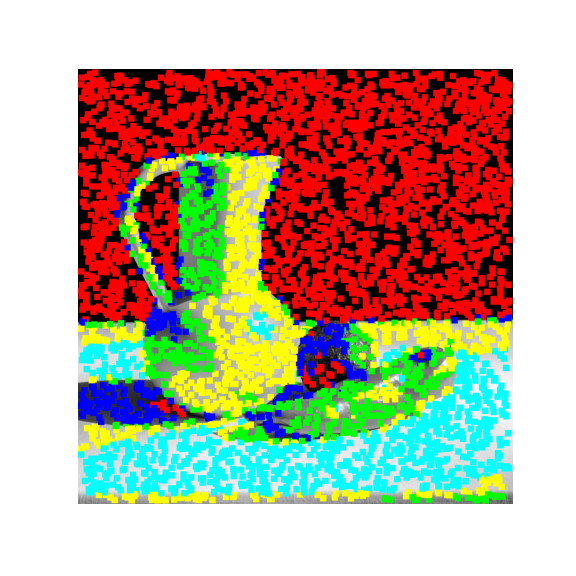
\includegraphics[scale=0.6]{images/window_colorized.png}
\caption{5000 darab, $15 \times 15$ px méretű ablak szegmentálása és megjelenítése az eredeti képen.}
\label{fig:window_colorized}
\end{figure}

\SubSection{Osztályozás/KNN}

\Section{Optimális klaszterszám meghatározása} \label{optimal_cluster_number}

Az optimális klaszterszám meghatározásához 4 módszert teszteltem le, ezeknek az eredménye a következő alfejezetekben található.
A módszereket a \cite{tomatoleaf} és a \cite{elbow} kutatások alapján választottam.

A módszereknél a klaszterekre bontás idejét nem veszem figyelembe, csak magának a módszernek a futási idejét.

\SubSection{Silhouette módszer}

A Silhouette index azt méri, hogy egy adott objektum mennyire hasonlít a saját klaszterében lévő objektumokhoz. Az értéke +1 és -1 között mozog. A nagyobb érték azt jelzi, hogy az objektum jól illeszkedik a saját klaszteréhez és rosszul illeszkedik a szomszédos klaszterekhez. Ha a legtöbb objektumnak pozitív az értéke akkor a klaszterezés megfelelő, ha sok objektumnak negatív akkor vagy túl sok, vagy túl kevés a klaszter.

A módszer a következő képlettel írható le:

\[ S(k)=\frac{1}{num} \sum_{i=1}^{num} \frac{b(i)-a(i)}{max\{a(i),b(i)\}} \quad \]

\noindent ahol
\begin{itemize}
\item $n$: a klaszterek száma
\item $num$: a pixelek száma
\item $a(i)$: az $i$ minta és az ugyanabban a klaszterben lévő többi minta közötti átlagos távolság
\item $b(i)$: az $i$ minta és az összes többi klaszter mintája közötti távolság minimális értéke
\end{itemize}
Ennek eredményeként megkapjuk a Silhouette pontszámot. Ha elvégezzük ezt a vizsgálatot különböző klaszterszámokra, akkor amelyiknek a pontszáma a legnagyobb, az lesz a legoptimálisabb klaszterszám. \cite{tomatoleaf}

Vizsgálataim során a \texttt{sklearn.metrics} csomagban található \texttt{silhouette\_score} módszert használtam a következő kódrészletben látható módon. Ez a metódus megtalálható az általam készített \texttt{commonmethods} csomagban.
\begin{python}
def silhouette_method(values, labels):
    """
    Calculating the Silhouette method for the given values with
    the given labels, and measuring time.
    :param values: in my case the pixel values from the k-means method
    :param labels: in my case the labels from the k-means method
    :return: the time of the calculation and
        the calculated Silhouette score
    """
    start = time.time()
    s_score = silhouette_score(values, labels)
    end = time.time()

    s_time = end-start

    return s_time, s_score
\end{python}
Mint látható, a metódus visszatér a módszer számítási idejével, mivel a vizsgálataim során a futási idők összevetése volt az egyik fő szempont. Ezen kívül visszaadja a kiszámított Silhouette pontszámot is, amit az általam megadott értékekből és a hozzájuk tartozó címkékből állít elő. Ezeket az értékeket a \texttt{kmeans\_segmentation} metódus eredményeként kapom.

A Silhouette módszer esetén azt tapasztaltam, hogy a futási ideje elég lassú. A \ref{fig:silhouette_runtime}. ábrán látható a módszer futási ideje különböző méretű képekre.

\begin{figure}[h]
\centering
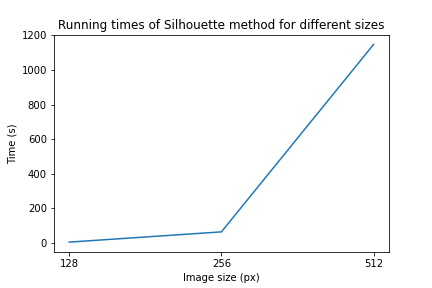
\includegraphics[scale=0.7]{images/silhouette_runtime.png}
\caption{A Silhouette módszer futási ideje különböző képméretekre.}
\label{fig:silhouette_runtime}
\end{figure}

Jól látható, hogy míg a 128px méretű képre pár másodperc alatt elvégzi a számítást, az 512px méretű képre már nagyságrendileg 20 percig számol.

\SubSection{Davies-Bouldin módszer}
A Davies-Bouldin index a klaszteren belüli szóródás összegének, és a klaszterek közötti szétválás arányának a függvénye. A célunk az hogy ezt az értéket minimalizáljuk, hiszen azt szeretnénk, hogy a klaszteren belüli szórás minimális, a klaszterek közötti elkülönülés pedig maximális legyen.

A módszer képlete a következő:

\[ DB(k)=\frac{1}{k} \sum_{i=1}^{K} max \left(\frac{W_i + W_j}{C_{ij}}\right)  \quad \]

\noindent ahol
\begin{itemize}
\item $K$: a klaszterek száma
\item $W_i$: a $C_i$ osztályba tartozó összes minta átlagos távolsága a klaszter középpontjától
\item $W_{j}$: a $C_i$ osztályba tartozó összes minta átlagos távolsága a $C_j$ osztály középpontjától
\item $C_{ij}$: a $C_i$ és $C_j$ osztályok középpontja közötti távolság
\end{itemize}
Ennek eredményeként megkapjuk a Davies-Bouldin pontszámot. Ha elvégezzük ezt a vizsgálatot különböző klaszterszámokra, akkor amelyiknek a pontszáma a legkisebb, az lesz a legoptimálisabb klaszterszám. \cite{tomatoleaf}

Ennek a módszernek a megvalósításához a \texttt{sklearn.metrics} csomagban található \texttt{davies\_bouldin\_score} metódust használtam. A következő kódrészletben látható, hogy a módszer megvalósítása ugyan arra a sémára épül, mint a \texttt{silhouette\_method}.

Ez a metódus is megtalálható az általam készített \texttt{commonmethods} csomagban.
\begin{python}
def davies_bouldin_method(values, labels):
    """
    Calculating the Davies-Bouldin method for the given values with
    the given labels, and measuring time.
    :param values: in my case the pixel values from the k-means method
    :param labels: in my case the labels from the k-means method
    :return: the time of the calculation and
        the calculated Davies-Bouldin score
    """
    start = time.time()
    db_score = davies_bouldin_score(values, labels)
    end = time.time()

    db_time = end-start

    return db_time, db_score
\end{python}

\SubSection{Calinski-Harabasz módszer}

A Calinski-Harabasz indexet belső klaszterérvényességi mérőszámként szokták használni, amely a létrehozott klasztereket osztályozza.

A módszer képlete a következő:

\begin{align*}
 CH(k) & =\frac{B(K)(N-K)}{W(K)(K-1)} \\
 B(K) & =\sum_{k=1}^{K}a_k \|\overline{x_k}-\overline{x}\|^2 \\
 W(K) & =\sum_{k=1}^{K}\sum_{C(j)=k}\|x_j-\overline{x_k}\|^2
\end{align*}

\noindent ahol
\begin{itemize}
\item $K$: a klaszterek száma
\item $N$: a minta száma
\item $B(K)$: a klaszterek közötti divergencia, más néven a klaszterek közötti kovariancia
\item $W(K)$: a klaszteren belüli divergencia, más néven a klaszteren belüli kovariancia
\end{itemize}

Minél nagyobb a $B(K)$ értéke, annál nagyobb a klaszterek közötti diszperzió mértéke. Minél kisebb a $W(K)$ értéke, annál szorosabb a kapcsolat a klaszteren belül. Minél nagyobb az arány, annál nagyobb a Calinski-Harabasz pontszám értéke, theát annál optimálisabb a klaszterszám. \cite{silhouette_calinski}

Ennek a módszernek a megvalósításához a \texttt{sklearn.metrics} csomagban található \texttt{calinski\_harabasz\_score} metódust használtam. A következő kódrészletben látható hogy, a módszer megvalósítása ugyan arra a sémára épül, mint a \texttt{silhouette\_method} és a \texttt{davies\_bouldin\_method}.

Ez a metódus is megtalálható az általam készített \texttt{commonmethods} csomagban.
\begin{python}
def calinski_harabasz_method(values, labels):
    """
    Calculating the Calinski-Harabasz method for the given values with
    the given labels, and measuring time.
    :param values: in my case the pixel values from the k-means method
    :param labels: in my case the labels from the k-means method
    :return: the time of the calculation and
        the calculated Calinski-Harabasz score
    """
    start = time.time()
    ch_score = calinski_harabasz_score(values, labels)
    end = time.time()

    ch_time = end-start
\end{python}

\SubSection{Elbow módszer}

Az Elbow módszer a variancia százalékos arányát vizsgálja a klaszterek számának függvényében. Azon az elven alapszik, hogy olyan klaszterszámot kell választanunk amelyhez ha hozzáadnánk akár csak egy klasztert is, akkor a modellünk már nem javulna számottevő mértékben.

Az első klaszterek sok információt adnak hozzá a modellhez, viszont egy bizonyos ponton a határnyereség drámaian lecsökken és szöget, vagyis könyököt képez a grafikonon (lásd. \ref{fig:elbow_grayscale}. ábra). Innen ered az "elbow" azaz "könyök" módszer elnevezés. Az a pont ahol ez a drámai csökkenés bekövetkezik, az lesz a megfelelő klaszterszám. A \ref{fig:elbow_grayscale}. ábrán ez a pont 2 klaszternél alakul ki, de érdemes lehet megvizsgálni a 3 klasztert is. \cite{elbow}

\begin{figure}[h]
\centering
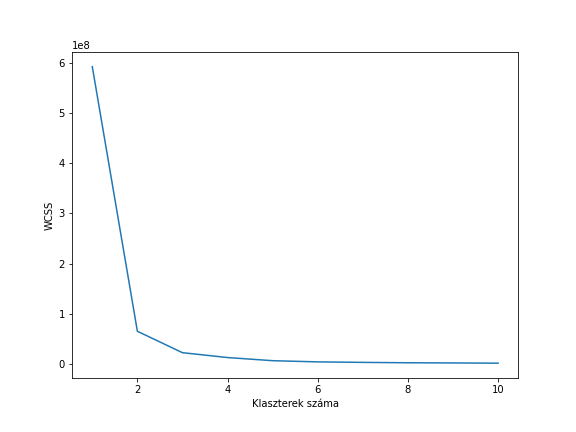
\includegraphics[scale=0.7]{images/elbow_grayscale.png}
\caption{Elbow módszer alkalmazása szürkeárnyalatos képre}
\label{fig:elbow_grayscale}
\end{figure}

Az Elbow metódushoz a \texttt{kmeans\_segmentation} által eredményként visszaadott \texttt{compactness} értékeket szükséges lementenünk különböző méretű klaszterekre ahogy az a következő kódrészletben látható.
\begin{python}
import commonmethods.image_modification as im

wcss = []   #within cluster sum of squares

for k in range(1, 11):
    compactness, _, _, _ = \
        im.kmeans_segmentation(resized_image, k)
    wcss.append(compactness)
\end{python}

Ha a \texttt{wcss} listát \texttt{plot} segítségével ábrázoljuk, meg is kaptuk az Elbow grafikonunkat pont úgy, mint ahogy a \ref{fig:elbow_grayscale}. ábrán szerepel.

Ennél a módszernél külön számítást nem kell végeznünk, így futási ideje igazából csak maga a kirajzolás.

Összességében a módszer gyors, viszont nem mindig ad egyértelmű eredményt és a töréspont automatizált meghatározása sem egy egyszerű feladat. Vizuális ábrázolásra és kézi ellenőrzésre viszont megfelelő, így főként én is erre a célra használtam.

\SubSection{Összegzés}

A módszerek vizsgálata során hamar kiderült, hogy a Silhouette módszer futási ideje számottevően nagyobb a többi módszerétől. Az eredmények összehasonlítását a \ref{tab:size_runtimes}. táblázat tartalmazza. Mivel az Elbow módszer nem egyértelmű és főként vizuális megerősítésként szolgál, így ezt a módszert kihagytam a további elemzésekből.

\begin{table}[h]
\centering
\caption{Futási idők átlaga különböző módszerek esetén}
\label{tab:size_runtimes}
\medskip
\begin{tabular}{|l|c|c|c|c|}
\cline{2-5}
 \multicolumn{1}{c|}{} & \multicolumn{4}{c|}{Kép mérete} \\
 \hline
 Módszer & 64px & 128px & 256px & 512px \\
\hline
Silhouette módszer & 0.2684s & 4.4029s & 68.0697s & 1183.2937s \\
Davies-Bouldin módszer & 0.0071s & 0.0042s & 0.0096s & 0.0274s \\
Calinski-Harabasz módszer & 0.0031s & 0.001s & 0.0028s & 0.0120s \\
\hline
\end{tabular}
\end{table}

A táblázat jól szemlélteti, hogy a Silhouette módszer futási ideje már a legkisebb képméretre is majdnem negyveszerese a másik két módszer futási idejének.

Mivel a klaszterek számának növelésével a feldolgozandó adathalmaz nem változik, így a klaszterek száma nem befolyásolja a módszerek futási idejét. Erre bizonyítékként szolgál a \ref{tab:cluster_runtimes}. táblázat amely különböző klaszterszám esetén mutatja be az átlagos futási időket. Jól látható hogy nem növekszik, sőt valahol csökken a magasabb klaszterszám esetén a futási idő.

\begin{table}[h]
\centering
\caption{Futási idők átlaga különböző klaszterszámok és módszerek esetén, 256px képméretre}
\label{tab:cluster_runtimes}
\medskip
\begin{tabular}{|l|c|c|c|}
\cline{2-4}
 \multicolumn{1}{c|}{} & \multicolumn{3}{c|}{Klaszterek száma} \\
 \hline
 Módszer & 2 & 4 & 8 \\
\hline
Silhouette módszer & 63.1462s & 63.1254s & 62.2278s \\
Davies-Bouldin módszer & 0.0060s & 0.0083s & 0.0064s \\
Calinski-Harabasz módszer & 0.0026s & 0.0024s & 0.0028s \\
\hline
\end{tabular}
\end{table}

Természetesen a K-means metódus lassabban határozza meg a klasztereket nagyobb klaszterszám esetén, így a nagyobb klaszterszám magának a programnak a futási idejét befolyásolja.

A futási idők mellett a módszerek jóságát is megvizsgáltam mind színes, mind szürkeárnyalatos képek esetén. Ennek a vizsgálatnak az eredményét a \ref{tab:cluster_result}. táblázatban foglaltam össze.

A módszereket minden képméretre több alkalommal is lefuttattam, ezekből a futások alkalmával kapott összes klaszterszámot megjelenítettem. Jól látható, hogy a Silhouette és a Davies-Bouldin módszer minden képméretre, minden futási alkalommal ugyanazt az eredményt szolgáltatta, és a két módszer eredményei megegyeznek.

Ezzel szemben a Calinski-Harabasz módszer eredménye eltér a másik 2 módszer eredményétől, és a különböző képméretekre más-más klaszterszámmal szolgált. Emelett még az is látható hogy egy azon képméret esetén, például a 64px méretű színes képnél több futás alkalmával más-más klaszterszámot adott eredményül.

\begin{table}[h]
\centering
\caption{Meghatározott klaszterszám különböző képméretek és módszerek esetén}
\label{tab:cluster_result}
\medskip
\begin{tabular}{|l|c|c|c|c|c|c|}
\cline{2-7}
 \multicolumn{1}{c|}{} & \multicolumn{6}{c|}{Kép mérete} \\
 \hline
 \multirow{2}{*}{Módszer} & \multicolumn{2}{c|}{64px} & \multicolumn{2}{c|}{126px} & \multicolumn{2}{c|}{256px} \\
 \cline{2-7}
 & Szürke & Színes & Szürke & Színes & Szürke & Színes  \\
\hline
Silhouette módszer & 2 & 3 & 2 & 3 & 2 & 3 \\
Davies-Bouldin módszer & 2 & 3 & 2 & 3 & 2 & 3 \\
Calinski-Harabasz módszer & 10 & 8,10 & 9,10 & 10 & 9 & 8,9 \\
\hline
\end{tabular}
\end{table}

Elvégeztem az Elbow módszert is a színes képre, ennek az eredménye a \ref{fig:elbow_rgb}. ábrán látható. A szürkeárnyalatos változatát a \ref{fig:elbow_grayscale}. ábra tartalmazza, ezt használtam fel példának az Elbow módszer bemutatásakor. Látható, hogy mind a két esetben a 2 és 3 klaszternél található meg törés a grafikonon, tehát az Elbow módszer is ezeket a klaszterszámokat javasolja.

\begin{figure}[h]
\centering
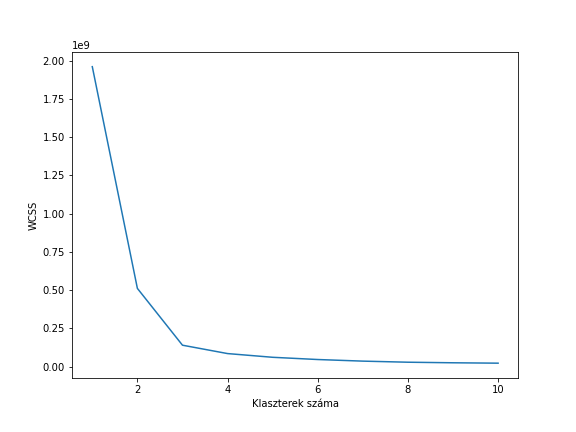
\includegraphics[scale=0.7]{images/elbow_rgb.png}
\caption{Elbow módszer alkalmazása színes képre}
\label{fig:elbow_rgb}
\end{figure}

A Módszerek által megadott klaszterszámokkal elvégeztem a klaszterezést, az eredmény a \ref{fig:kmeans_optimal_pictures}. ábrán látható.

\begin{figure}[h]
\centering
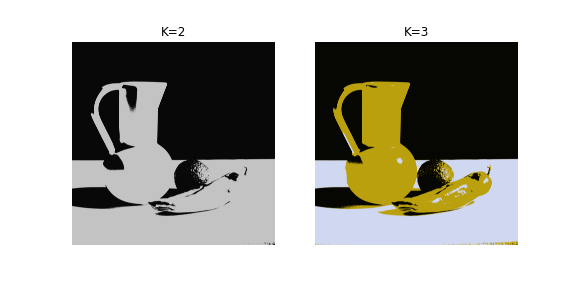
\includegraphics[scale=0.7]{images/kmeans_optimal_pictures.png}
\caption{K-means klaszterezés a módszerek által megadott optimális klaszterszámmal}
\label{fig:kmeans_optimal_pictures}
\end{figure}

Összegezve a vizsgálatokat ki lehet jelenteni, hogy a legjobb módszer az optimális klaszterszám meghatározására a vizsgáltak közül az a Davies-Bouldin módszer.

A Silhouette-módszer igaz hogy pontos, de a futási ideje nagyon magas. Ha egészen kis méretű képeket használunk akkor talán még alkalmazható, de nagyobb képek esetén nagyon megnöveli a program futási idejét.

A Calinski-Harabasz módszer futási ideje sok esetben jobb volt, mint a Davies-Bouldin módszeré, viszont a klaszterszám meghatározása nagyon pontatlan. Egyszer sem szolgáltatta azt az eredményt amit a másik három módszerből kaptam. 
\Chapter{Szürkeárnyalatos képek kiszínezése}

A szürkeárnyalatos kép és a megkapott címke térkép segítségével már az előző fejezetben ki tudtuk színezni a szegmenseket, viszont a kiszínezés az eredeti kép árnyalatait nem vette figyelembe. A fejezet célja hogy a színezést úgy valósítsuk meg, hogy az eredeti kép árnyalatait is megjelenítjük. A minél jobb eredmény elérésének érdekében az RGB és HSV színterekben is megvizsgáltam a problémát, ezeknek a vizsgálatoknak az eredménye a következő alfejezetekben található.

Maguk a színterek a színek matematikai ábrázolásai, lehetővé teszik a színek reprodukálható geometriai ábrázolását a 2D-3D terekben. A színterek a színmodellek és a leképezési függvények kombinációja, és információt tartalmaznak a kép egyes pixeleinek a színéről. A színes képek szegmentálására használt gyakori színterek az RGB, YIQ, HSV, CIE XYZ. \cite{colorspaces}

\Section{RGB}

Az RGB színterű képekben a kép minden egyes pixelét 3 színnel határozzuk meg:
\begin{itemize}
\item vörös (Red)
\item zöld (Green)
\item kék (Blue)
\end{itemize}
A paraméterek a szín intenzitását határozzák meg, az értékük egy 0-255 közötti egész szám. Ha mindegyik paraméterből a maximális, 255 értéket vesszük akkor a fehér színt, ha mindegyikből a minimális, az az a 0 értéket vesszük, akkor pedig a fekete színt kapjuk meg.  Egyszerűsége miatt a színtér széles körben elterjedt. \cite{colorspaces}

Szürkeárnyalatos képek esetén a 3 paraméter értéke megegyezik, így legtöbb esetben csak 1 értékkel szokták a kép pixeleit jelölni, tehát például szürkeárnyalatos képnél egy fekete színű pixel értéke 0.

Ahhoz, hogy egy szürkeárnyalatos képen színt tudjunk megjeleníteni, először át kell alakítanunk RGB színterűvé. Az átalakítást, hasonlóan az előző fejezetben bemutatott \texttt{color\_image} függvényhez, a \texttt{cv2} csomag \texttt{cvtColor} metódusával fogjuk megtenni.
\begin{python}
colored_image = cv2.cvtColor(resized_image, cv2.COLOR_GRAY2RGB)
\end{python}

Egy adott pixelre a színt a következő képlettel határozom meg:
\begin{align*}
 \text{new\_pixel\_color} & = (R, G, B) \\
 Y & = \text{grayscale\_image}[i][j]\\
 R_{ij} & = Y \cdot R / 255 \\
 G_{ij} & = Y \cdot G / 255 \\
 B_{ij} & = Y \cdot B / 255 \\
 \text{colored\_image}_{ij} & = (R_{ij}, G_{ij}, B_{ij})
\end{align*}
\noindent ahol az $i,j$ a kép adott pixelének az indexe.

A pixeleket a \texttt{numpy} csomag \texttt{multiply} függvényével színezem ki a következő kódrészletben látható módon.

\begin{python}
r, g, b = cv2.split(colored_image)

for i in range(0, k):
    np.multiply(r, colors[i][0]/255, out=r,
                where=label_map==i, casting="unsafe")
    np.multiply(g, colors[i][1]/255, out=g,
                where=label_map==i, casting="unsafe")
    np.multiply(b, colors[i][2]/255, out=b,
                where=label_map==i, casting="unsafe")

colored_image = cv2.merge([r, g, b])
\end{python}

Első lépésként a képet a \texttt{cv2.split} segítségével szétválasztom R, G és B komponensekre. Eredményül 3 tömböt kapok, amik az eredeti pixel adott paraméterét tartalmazzák. Ezeken a tömbökön for ciklus segítségével is végig iterálhatnék, és megadhatnám minden pixelnek az értékét a fentebb említett képlet alapján, viszont a \texttt{numpy} csomag \texttt{multiply} függvénye ezt a szorzást sokkal gyorsabban elvégzi. A klaszterek számán haladok végig, ami tulajdonképpen a címkék értékét jelenti és minden címkére elvégzem a szorzást.

A \texttt{multiply} függvény első 2 paramétereként a szorzás 2 tényezőjét várja. Első elemnek az adott komponens tömböt adom meg, második elemnek pedig a címke által meghatározott szín megfelelő komponensének a 255-el osztott értékét. A \texttt{colors} tömb megegyezik a már korábban bemutatott \texttt{color\_image} függvényben található azonos nevű tömbbel.

A művelet kimeneti értékének ugyanazt a tömböt adom meg. A szorzásnak megadok egy \texttt{where} feltételt, ahol a címke térkép adott elemét fogja vizsgálni a metódus. Megnézi, hogy az adott címke értéke megegyzik-e az éppen vizsgált címkének az értékével és ha igen, csak akkor végzi el a szorzást, tehát csak akkor színezi ki a pixelt.

Utolsó paraméterként a \texttt{casting} paraméternek unsafe értéket állítok be, ez azt jelenti, hogy a nem egyforma típusú értékek esetén is elvégzi a szorzást a függvény.

A szorzások után már csak össze kell olvasztanom a 3 különálló tömböt. Ez a \texttt{cv2.merge} függvénnyel egyszerűen megtudom valósítani. A színezésre példa a \ref{fig:colorized_rgb}.ábrán látható.

\begin{figure}[h]
\centering
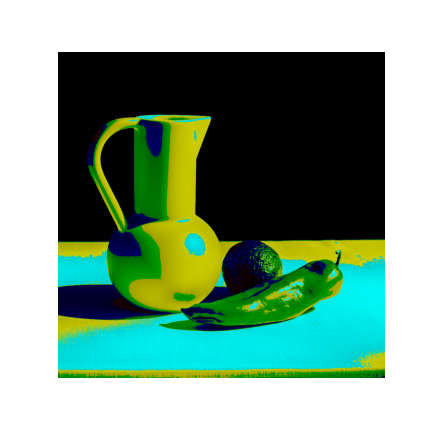
\includegraphics[scale=0.7]{images/colorized_rgb.png}
\caption{Szürkeárnyalatos kép kiszínezése RGB színtérben.}
\label{fig:colorized_rgb}
\end{figure}

Itt már szépen megjelennek az árnyékok, jól kivehetőek a színátmenetek.

\Section{HSV}

A HSV színtér szintén széles körben használt, az emberi szem számára megfelelőbb színtér. A HSV színtérben minden pixelt a következő 3 paraméter határoz meg:
\begin{itemize}
\item színárnyalat (Hue)
\item telítettség (Saturation)
\item érték (Value)
\end{itemize}

A színárnyalat (H) az alapszínt jelöli vagy fokban, vagy számokban. A színek skáláját a \ref{tab:hsv_colors}. táblázat szemlélteti.

\begin{table}[h]
\centering
\caption{HSV színtér színárnyalatainak az értéke.}
\label{tab:hsv_colors}
\medskip
\begin{tabular}{|c|c|c|}
\hline
Érték fokban & Érték számmal & Értékhez tartozó szín \\
\hline
0$^{\circ}$ vagy 360$^{\circ}$ & 0 vagy 6 & Vörös \\
\hline
60$^{\circ}$ & 1 & Sárga \\
\hline
120$^{\circ}$ & 2 & Zöld \\
\hline
180$^{\circ}$ & 3 & Cián \\
\hline
240$^{\circ}$ & 4 & Kék \\
\hline
300$^{\circ}$ & 5 & Magenta \\
\hline
\end{tabular}
\end{table}

A telítettség (S) azt írja le, hogy a szín milyen mennyiségben tartalmazza a fehér színt. A telítettséget mindig százalékos értékben adjuk meg, a 100\% jelenti a teljesen telített színt. Minél kisebb az értéke, annál halványabb a szín, mivel egyre több szürkét tartalmaz.

Az értéket (V) szokták fényerőnek (Brightness) is hívni, olyankor a színteret HSB színtérként emlegetik, de ez megegyezik a HSV színtérrel. A az érték a szín sötétségét fejezi ki százalékos arányban, ahol a 0\% a fekete, a 100\% a fehér színt jelenti. \cite{colorspaces}

A HSV színtérben található szürkeárnyalatos képek a H és S csatornákon 0 értékeket tartalmaznak, a kép csak a V értékeiből áll. Ahhoz, hogy szürkeárnyalatosból színes képet tudjunk készíteni, szükségünk van mind a H és mind az S csatorna értékeire. A \ref{fig:hsv_colorization}. ábra szemlélteti a színezés megvalósításának lehetőségeit.

\begin{figure}[h]
\centering
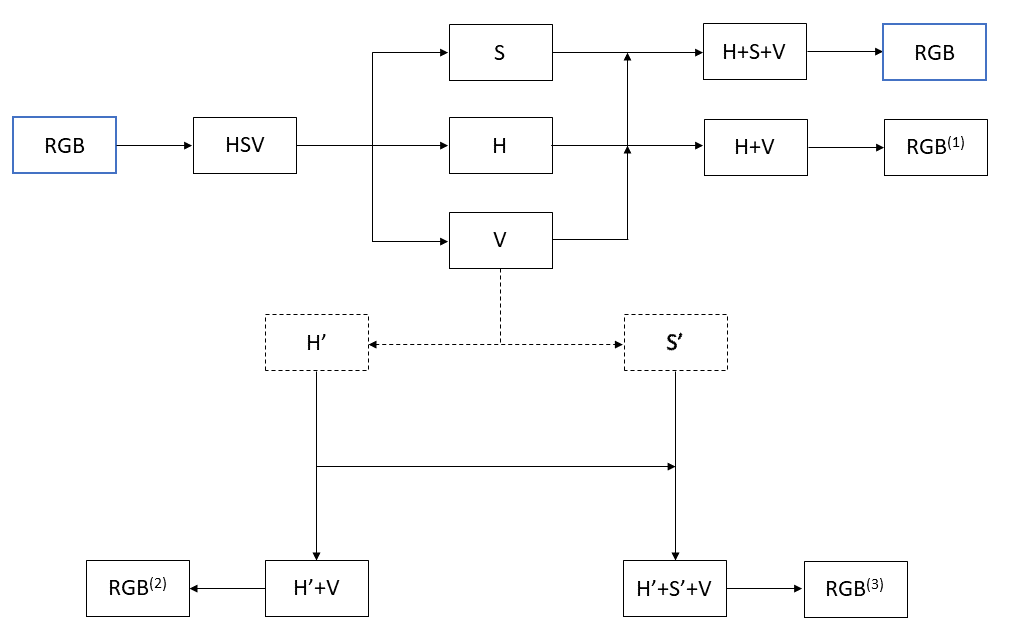
\includegraphics[scale=0.5]{images/hsv_colorization.png}
\caption{Kép színének visszabecslése HSV színtérben.}
\label{fig:hsv_colorization}
\end{figure}

Az ábra abból indul ki hogy van egy RGB színterű képünk, ezt átalakítjuk HSV színterűvé. Ha csatornáira bontjuk a képet, akkor a V  jelzi nekünk a szürkeárnyalatos képet. Amennyiben ismerjük az eredeti H és S csatornákat, akkor jól látható, hogy az eredeti képet fogjuk visszakapni. Amennyiben csak a H értékeit ismerjük, abban az esetben az $RGB^{(1)}$ kép elég hasonló, de színerősségben nagy valószínűséggel különböző lesz. Ezek azok az esetek, amikor valahonnan visszakapjuk ezeket az értékeket, például ha egyébként megvan az eredeti RGB kép és onnan meghatározzuk őket.

Amennyiben csak egy szürkeárnyalatos képünk van, abban az esetben ezeket a csatornákat valahogyan meg kell becsülnünk. Az ábrán a szaggatott vonal jelképezi a becslést, a becsült csatornákat pedig H' és S' jelöli.

Amennyiben a H csatornát tudjuk csak megbecsülni, abban az esetben az S értékének valamilyen átlagértéket veszünk. A kapott $RGB^{(2)}$ képünk nagyban el fog térni az eredeti képtől, hiszen a színek sem biztos hogy pontosak, az árnyalatuk pedig csak egy meghatározott átlag érték, tehát ha az eredeti kép nagyon erős színeket tartalmaz vagy nagyon halvány színeket, akkor az eredmény képünk nagyon eltérő lesz tőle.

Amennyiben viszont az S értékét is vissza tudjuk becsülni, abban az esetben az $RGB^{(3)}$ valószínűleg annyira pontos nem lesz, mintha meglenne az eredeti H és S csatorna, viszont pontosabb lesz mint az $RGB^{(1)}$ illetve az $RGB^{(2)}$.

A \texttt{colors} tömb felhasználásával egyszerűen ki lehet színezni egy szürkeárnyalatos HSV színterű képet. Az RGB színeket átalakítva HSV színterű színekké megkapjuk a H, illetve az S értékét is a színnek. Ezután már csak annyi dolgunk van, hogy ezeket az értékeket átadjuk az összes pixelnek. Egy ilyen színezés megvalósításának a kódja látható a következő kódrészletben.
\begin{python}
import colorsys

colored_image_rgb = cv2.cvtColor(resized_image, cv2.COLOR_GRAY2RGB)

hsv_image = cv2.cvtColor(colored_image_rgb, cv2.COLOR_RGB2HSV)

colored_hsv = hsv_image

for label in range(k):
    color_hsv = colorsys.rgb_to_hsv(
        colors[label][0]/255,
        colors[label][1]/255,
        colors[label][2]/255)
    for i in range(1024):
        for j in range(1024):
            if(label_map[i][j] == label):
                colored_hsv[i][j] =\
                [color_hsv[0]*180, color_hsv[1]*255, hsv_image[i][j][2]]
\end{python}

A színek konvertálására a \texttt{colorsys} csomagot használom, abból is az \texttt{rgb\_to\_hsv} függvényt, ami bemenetként az RGB szín csatornáit várja 0 és 1 közötti értékként, ezért a szín minden értékét el kell osztani 255-tel. A meglévő szürkeárnyalatos képet átalakítom színes képpé a már korábban bemutatott módon, majd a színes képet HSV színterűvé. Ezután indítok egy for ciklust a k értékein, ami csak úgy, mint az RGB színezésnél a label értékeket fogja jelölni. Ezután a \texttt{colors} tömbből megkapott RGB színt átkonvertálom HSV színné. Minden olyan pixelt, ami a \texttt{label\_map} szerint az éppen vizsgált label értékű, kiszínezek a megadott szín szerint. A konvertálás során a HSV szín értékei 0 és 1 közötti értékek lettek, így ezeket még fel kell szorozni, hogy a megfelelő színeket kapjuk. A V értéke mindenhol marad az eredeti, szürkeárnyalatos kép V értéke.

A színezés eredménye a \ref{fig:colorized_hsv}. ábrán látható.

\begin{figure}[h]
\centering
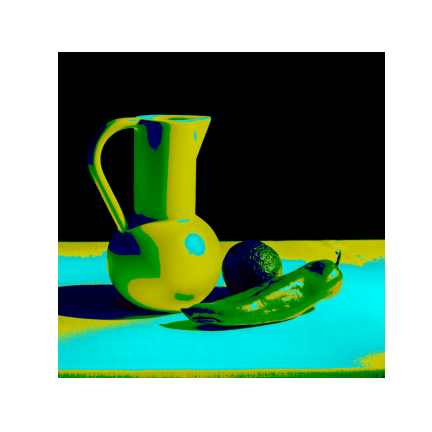
\includegraphics[scale=0.7]{images/colorized_hsv.png}
\caption{Szürkeárnyalatos kép kiszínezése HSV színtérben.}
\label{fig:colorized_hsv}
\end{figure}

A képet a kiszínezés után az egyszerű kirajzolás érdekében visszaalakítottam RGB színterűvé. Jól látható, hogy a két színtérben történő színezés ugyanazt a képet eredményezi.

\Section{Képek színének visszabecslése}

Az előző alfejezetekben bemutatott színezés során a kép színeit általam előre meghatározott színekből, random választottam ki.
\Chapter{A vizsgálatokhoz készített programok}

Ahogy már a korábbi fejezetekben említettem, a dolgozathoz Python programozási nyelvet használtam. A vizsgálatokhoz elsősorban Jupyter munkafüzeteket készítettem, majd a vizsgálatok lezárultával ezeket a kódrészleteket összefoglaltam Python fileokba, és készítettem belőlük egy különálló programot.

A fő program és a notebookok futtatásához a következő függőségek szükségesek:
\begin{itemize}
\item NumPy
\item OpenCv
\item Matplotlib
\item Scikit-learn
\item Scikit-image
\item Tensorflow
\item Az általam készített commonmethods
\end{itemize}


\Chapter{Tesztelés}

A fejezetben be kell mutatni, hogy az elkészült alkalmazás hogyan használható.
(Az, hogy hogyan kell, hogy működjön, és hogy hogy lett elkészítve, az előző fejezetekben már megtörtént.)

Jellemzően az alábbi dolgok kerülhetnek ide.
\begin{itemize}
\item Tesztfuttatások. Le lehet írni a futási időket, memória és tárigényt.
\item Felhasználói kézikönyv jellegű leírás. Kifejezetten a végfelhasználó szempontjából lehet azt bemutatni, hogy mit hogy lehet majd használni.
\item Kutatás kapcsán ide főként táblázatok, görbék és egyéb részletes összesítések kerülhetnek.
\end{itemize}

\Chapter{Összegzés}

Hasonló szerepe van, mint a bevezetésnek.
Itt már múltidőben lehet beszélni.
A szerző saját meglátása szerint kell összegezni és értékelni a dolgozat fontosabb eredményeit.
Meg lehet benne említeni, hogy mi az ami jobban, mi az ami kevésbé jobban sikerült a tervezettnél.
El lehet benne mondani, hogy milyen további tervek, fejlesztési lehetőségek vannak még a témával kapcsolatban.

\Chapter{Summary}

The content of the previous chapter in english.

\clearpage

\addcontentsline{toc}{chapter}{Irodalomjegyzék}
\bibliographystyle{unsrt}
\bibliography{dolgozat}

\noindent \textit{Az internetes források utolsó ellenőrzése: 2021.10.05}

\pagestyle{empty}

\newpage

\pagestyle{empty}

\noindent \textbf{\Large CD melléklet tartalma}

\vskip 1cm

\noindent A dolgozathoz mellékelt lemezen egy \texttt{Dolgozat} nevű jegyzékben a következő fájlok találhatóak.

\begin{itemize}
\item A dolgozat \LaTeX\ forráskódja.
\item A dolgozat PDF formátumban (\texttt{dolgozat.pdf}).
\item A magyar és angol nyelvű összefoglaló \LaTeX\ és PDF formátumban \\ (\texttt{osszegzes.tex}, \texttt{osszegzes.pdf}, \texttt{summary.tex}, \texttt{summary.pdf}).
\end{itemize}

Az \texttt{images} nevű jegyzékben találhatóak a vizsgálatokhoz használt mintaképek.

A \texttt{notebooks} jegyzékbe kerültek a dolgozat megírása során elkészített és az abban részletezett Jupyter munkafüzetek.

A \texttt{program} nevű jegyzékben található a dolgozathoz Python szkriptekként elkészített programok.


\end{document}
